\documentclass[tikz,border=10pt]{standalone}
\usepackage[T1]{fontenc}
\usepackage{helvet}
\renewcommand{\familydefault}{\sfdefault}
\usepackage{amsmath,amssymb}
\usepackage{tikz}
\usetikzlibrary{calc,positioning,fit,arrows.meta,shapes.geometric}

% Canonical Academic Palette
\definecolor{OxfordNavy}{HTML}{1E293B}
\definecolor{SlateSteel}{HTML}{334155}
\definecolor{MutedTeal}{HTML}{0F766E}
\definecolor{TealL0}{HTML}{F0FDFA}
\definecolor{Burgundy}{HTML}{991B1B}
\definecolor{BurgundyL0}{HTML}{FEF2F2}
\definecolor{WarmOchre}{HTML}{92400E}
\definecolor{OchreL0}{HTML}{FFFBEB}
\definecolor{ForestSage}{HTML}{166534}
\definecolor{SageL0}{HTML}{F0FDF4}
\definecolor{CoolParchment}{HTML}{F8FAFC}
\definecolor{SlateRim}{HTML}{CBD5E1}
\definecolor{GridGray}{HTML}{E2E8F0}
\definecolor{DarkSlate}{HTML}{0F172A}

\begin{document}
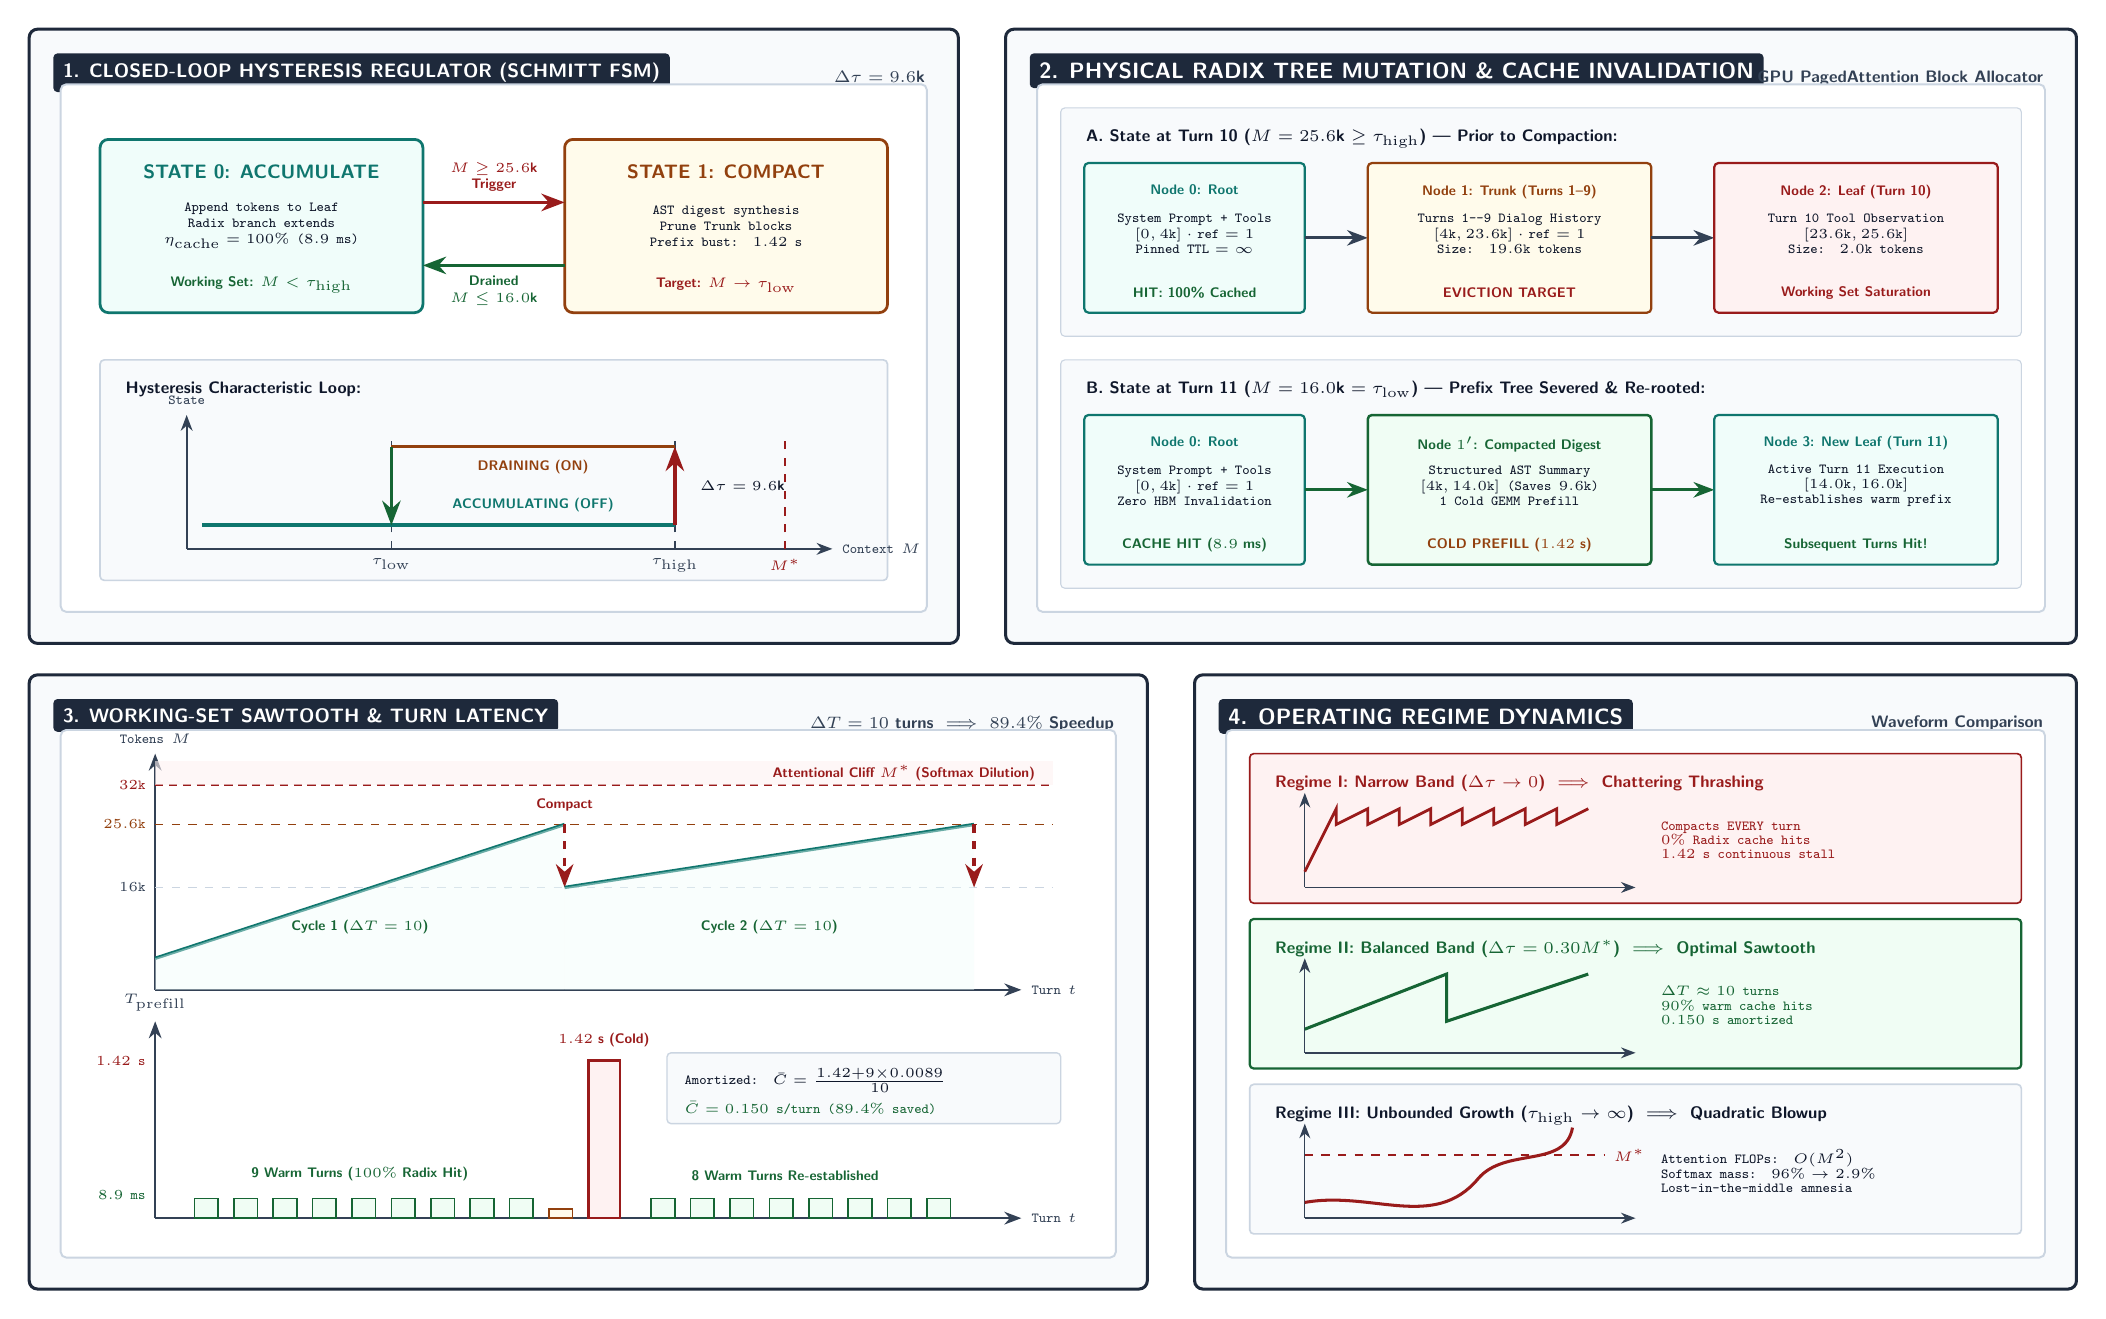
\begin{tikzpicture}[
  font=\sffamily,
  scale=1.0,
  >=Stealth,
  node distance=0.5cm
]

% =============================================================================
% TOP-LEFT (PANEL 1): CLOSED-LOOP HYSTERESIS REGULATOR (SCHMITT FSM)
% =============================================================================
\begin{scope}[shift={(0, 8.2)}]
  \draw[fill=CoolParchment, draw=OxfordNavy, line width=1.1pt, rounded corners=3pt]
    (0, 0) rectangle (11.8, 7.8);

  \node[anchor=north west, fill=OxfordNavy, text=white, font=\fontsize{7.5}{9.0}\selectfont\bfseries, rounded corners=1.5pt, inner sep=3.5pt]
    at (0.3, 7.5) {1. CLOSED-LOOP HYSTERESIS REGULATOR (SCHMITT FSM)};
  \node[anchor=north east, text=SlateSteel, font=\fontsize{5.8}{7}\selectfont\bfseries]
    at (11.5, 7.4) {$\Delta \tau = 9.6\text{k}$};

  \begin{scope}[shift={(0.4, 0.4)}]
    \draw[fill=white, draw=SlateRim, line width=0.7pt, rounded corners=2pt] (0, 0) rectangle (11.0, 6.7);

    % FSM State 0: ACCUMULATING
    \draw[fill=TealL0, draw=MutedTeal, line width=1.0pt, rounded corners=3pt] (0.5, 3.8) rectangle (4.6, 6.0);
    \node[anchor=north, font=\fontsize{6.8}{8}\selectfont\bfseries, text=MutedTeal] at (2.55, 5.8) {STATE 0: ACCUMULATE};
    \node[font=\fontsize{5.0}{5.8}\selectfont\ttfamily, text=DarkSlate, align=center] at (2.55, 4.9) {Append tokens to Leaf\\Radix branch extends\\$\eta_{\mathrm{cache}} = 100\%$ ($8.9\text{ ms}$)};
    \node[font=\fontsize{4.6}{5.2}\selectfont\bfseries, text=ForestSage] at (2.55, 4.15) {Working Set: $M < \tau_{\mathrm{high}}$};

    % FSM State 1: COMPACTING
    \draw[fill=OchreL0, draw=WarmOchre, line width=1.0pt, rounded corners=3pt] (6.4, 3.8) rectangle (10.5, 6.0);
    \node[anchor=north, font=\fontsize{6.8}{8}\selectfont\bfseries, text=WarmOchre] at (8.45, 5.8) {STATE 1: COMPACT};
    \node[font=\fontsize{5.0}{5.8}\selectfont\ttfamily, text=DarkSlate, align=center] at (8.45, 4.9) {AST digest synthesis\\Prune Trunk blocks\\Prefix bust: $1.42\text{ s}$};
    \node[font=\fontsize{4.6}{5.2}\selectfont\bfseries, text=Burgundy] at (8.45, 4.15) {Target: $M \to \tau_{\mathrm{low}}$};

    % Forward Transition: M >= tau_high
    \draw[->, draw=Burgundy, line width=1.2pt] (4.6, 5.2) -- (6.4, 5.2)
      node[midway, above, font=\fontsize{5.0}{6}\selectfont\bfseries, text=Burgundy, align=center] {$M \ge 25.6\text{k}$\\\fontsize{4.2}{5}\selectfont Trigger};

    % Backward Transition: M <= tau_low
    \draw[->, draw=ForestSage, line width=1.2pt] (6.4, 4.4) -- (4.6, 4.4)
      node[midway, below, font=\fontsize{5.0}{6}\selectfont\bfseries, text=ForestSage, align=center] {\fontsize{4.2}{5}\selectfont Drained\\$M \le 16.0\text{k}$};

    % Schmitt Trigger Transfer Function Graphic
    \draw[fill=CoolParchment, draw=SlateRim, line width=0.6pt, rounded corners=1.5pt] (0.5, 0.4) rectangle (10.5, 3.2);
    \node[anchor=north west, font=\fontsize{5.8}{7}\selectfont\bfseries, text=DarkSlate] at (0.7, 3.05) {Hysteresis Characteristic Loop:};

    % Inner axes
    \draw[->, draw=SlateSteel, line width=0.6pt] (1.6, 0.8) -- (9.8, 0.8)
      node[right, font=\fontsize{4.8}{5.5}\selectfont\ttfamily, text=SlateSteel] {Context $M$};
    \draw[->, draw=SlateSteel, line width=0.6pt] (1.6, 0.8) -- (1.6, 2.5)
      node[above, font=\fontsize{4.8}{5.5}\selectfont\ttfamily, text=SlateSteel] {State};

    % Loop path
    \draw[draw=SlateSteel, line width=0.5pt, dashed] (4.2, 0.8) -- (4.2, 2.2) node[below=1.4cm, font=\fontsize{4.8}{5.5}\selectfont\ttfamily, text=SlateSteel] {$\tau_{\mathrm{low}}$};
    \draw[draw=SlateSteel, line width=0.5pt, dashed] (7.8, 0.8) -- (7.8, 2.2) node[below=1.4cm, font=\fontsize{4.8}{5.5}\selectfont\ttfamily, text=SlateSteel] {$\tau_{\mathrm{high}}$};
    \draw[draw=Burgundy, line width=0.5pt, dashed] (9.2, 0.8) -- (9.2, 2.2) node[below=1.4cm, font=\fontsize{4.8}{5.5}\selectfont\ttfamily, text=Burgundy] {$M^*$};

    % Hysteresis loop trajectory
    \draw[draw=MutedTeal, line width=1.3pt] (1.8, 1.1) -- (7.8, 1.1);
    \draw[->, draw=Burgundy, line width=1.3pt] (7.8, 1.1) -- (7.8, 2.1);
    \draw[draw=WarmOchre, line width=1.3pt] (7.8, 2.1) -- (4.2, 2.1);
    \draw[->, draw=ForestSage, line width=1.3pt] (4.2, 2.1) -- (4.2, 1.1);

    % State Labels on loop
    \node[anchor=south, font=\fontsize{4.6}{5.5}\selectfont\bfseries, text=MutedTeal] at (6.0, 1.15) {ACCUMULATING (OFF)};
    \node[anchor=north, font=\fontsize{4.6}{5.5}\selectfont\bfseries, text=WarmOchre] at (6.0, 2.05) {DRAINING (ON)};
    \node[anchor=west, font=\fontsize{4.6}{5.5}\selectfont\bfseries, text=DarkSlate] at (8.0, 1.6) {$\Delta \tau = 9.6\text{k}$};

  \end{scope}
\end{scope}

% =============================================================================
% TOP-RIGHT (PANEL 2): RADIX TREE PREFIX CACHE MUTATION
% =============================================================================
\begin{scope}[shift={(12.4, 8.2)}]
  \draw[fill=CoolParchment, draw=OxfordNavy, line width=1.1pt, rounded corners=3pt]
    (0, 0) rectangle (13.6, 7.8);

  \node[anchor=north west, fill=OxfordNavy, text=white, font=\fontsize{8.0}{9.5}\selectfont\bfseries, rounded corners=1.5pt, inner sep=3.5pt]
    at (0.3, 7.5) {2. PHYSICAL RADIX TREE MUTATION \& CACHE INVALIDATION};
  \node[anchor=north east, text=SlateSteel, font=\fontsize{6.0}{7}\selectfont\bfseries]
    at (13.3, 7.4) {GPU PagedAttention Block Allocator};

  \begin{scope}[shift={(0.4, 0.4)}]
    \draw[fill=white, draw=SlateRim, line width=0.7pt, rounded corners=2pt] (0, 0) rectangle (12.8, 6.7);

    % Sub-panel A: Pre-Compaction Tree (Turn 10)
    \draw[fill=CoolParchment, draw=SlateRim, rounded corners=1.5pt] (0.3, 3.5) rectangle (12.5, 6.4);
    \node[anchor=north west, font=\fontsize{5.8}{7}\selectfont\bfseries, text=DarkSlate] at (0.5, 6.25) {A. State at Turn 10 ($M = 25.6\text{k} \ge \tau_{\mathrm{high}}$) --- Prior to Compaction:};

    % Node 0: Root
    \draw[fill=TealL0, draw=MutedTeal, line width=0.8pt, rounded corners=1.5pt] (0.6, 3.8) rectangle (3.4, 5.7);
    \node[anchor=north, font=\fontsize{5.5}{6.5}\selectfont\bfseries, text=MutedTeal] at (2.0, 5.55) {Node 0: Root};
    \node[font=\fontsize{4.8}{5.5}\selectfont\ttfamily, text=DarkSlate, align=center] at (2.0, 4.8) {System Prompt + Tools\\$[0, 4\text{k}] \cdot \text{ref}=1$\\Pinned $\text{TTL}=\infty$};
    \node[font=\fontsize{4.4}{5.2}\selectfont\bfseries, text=ForestSage] at (2.0, 4.05) {HIT: 100\% Cached};

    % Arrow Root -> Trunk
    \draw[->, draw=SlateSteel, line width=1.0pt] (3.4, 4.75) -- (4.2, 4.75);

    % Node 1: Trunk
    \draw[fill=OchreL0, draw=WarmOchre, line width=0.8pt, rounded corners=1.5pt] (4.2, 3.8) rectangle (7.8, 5.7);
    \node[anchor=north, font=\fontsize{5.5}{6.5}\selectfont\bfseries, text=WarmOchre] at (6.0, 5.55) {Node 1: Trunk (Turns 1--9)};
    \node[font=\fontsize{4.8}{5.5}\selectfont\ttfamily, text=DarkSlate, align=center] at (6.0, 4.8) {Turns 1--9 Dialog History\\$[4\text{k}, 23.6\text{k}] \cdot \text{ref}=1$\\Size: $19.6\text{k}$ tokens};
    \node[font=\fontsize{4.4}{5.2}\selectfont\bfseries, text=Burgundy] at (6.0, 4.05) {EVICTION TARGET};

    % Arrow Trunk -> Leaf
    \draw[->, draw=SlateSteel, line width=1.0pt] (7.8, 4.75) -- (8.6, 4.75);

    % Node 2: Leaf
    \draw[fill=BurgundyL0, draw=Burgundy, line width=0.8pt, rounded corners=1.5pt] (8.6, 3.8) rectangle (12.2, 5.7);
    \node[anchor=north, font=\fontsize{5.5}{6.5}\selectfont\bfseries, text=Burgundy] at (10.4, 5.55) {Node 2: Leaf (Turn 10)};
    \node[font=\fontsize{4.8}{5.5}\selectfont\ttfamily, text=DarkSlate, align=center] at (10.4, 4.8) {Turn 10 Tool Observation\\$[23.6\text{k}, 25.6\text{k}]$\\Size: $2.0\text{k}$ tokens};
    \node[font=\fontsize{4.4}{5.2}\selectfont\bfseries, text=Burgundy] at (10.4, 4.05) {Working Set Saturation};


    % Sub-panel B: Post-Compaction Tree (Turn 11)
    \draw[fill=CoolParchment, draw=SlateRim, rounded corners=1.5pt] (0.3, 0.3) rectangle (12.5, 3.2);
    \node[anchor=north west, font=\fontsize{5.8}{7}\selectfont\bfseries, text=DarkSlate] at (0.5, 3.05) {B. State at Turn 11 ($M = 16.0\text{k} = \tau_{\mathrm{low}}$) --- Prefix Tree Severed \& Re-rooted:};

    % Node 0: Root (Preserved)
    \draw[fill=TealL0, draw=MutedTeal, line width=0.8pt, rounded corners=1.5pt] (0.6, 0.6) rectangle (3.4, 2.5);
    \node[anchor=north, font=\fontsize{5.5}{6.5}\selectfont\bfseries, text=MutedTeal] at (2.0, 2.35) {Node 0: Root};
    \node[font=\fontsize{4.8}{5.5}\selectfont\ttfamily, text=DarkSlate, align=center] at (2.0, 1.6) {System Prompt + Tools\\$[0, 4\text{k}] \cdot \text{ref}=1$\\Zero HBM Invalidation};
    \node[font=\fontsize{4.4}{5.2}\selectfont\bfseries, text=ForestSage] at (2.0, 0.85) {CACHE HIT ($8.9\text{ ms}$)};

    % Arrow Root -> Compacted Trunk
    \draw[->, draw=ForestSage, line width=1.0pt] (3.4, 1.55) -- (4.2, 1.55);

    % Node 1': Compacted Digest
    \draw[fill=SageL0, draw=ForestSage, line width=0.9pt, rounded corners=1.5pt] (4.2, 0.6) rectangle (7.8, 2.5);
    \node[anchor=north, font=\fontsize{5.5}{6.5}\selectfont\bfseries, text=ForestSage] at (6.0, 2.35) {Node $1'$: Compacted Digest};
    \node[font=\fontsize{4.8}{5.5}\selectfont\ttfamily, text=DarkSlate, align=center] at (6.0, 1.6) {Structured AST Summary\\$[4\text{k}, 14.0\text{k}]$ (Saves $9.6\text{k}$)\\1 Cold GEMM Prefill};
    \node[font=\fontsize{4.4}{5.2}\selectfont\bfseries, text=WarmOchre] at (6.0, 0.85) {COLD PREFILL ($1.42\text{ s}$)};

    % Arrow Compacted Trunk -> New Leaf
    \draw[->, draw=ForestSage, line width=1.0pt] (7.8, 1.55) -- (8.6, 1.55);

    % Node 3: New Leaf
    \draw[fill=TealL0, draw=MutedTeal, line width=0.8pt, rounded corners=1.5pt] (8.6, 0.6) rectangle (12.2, 2.5);
    \node[anchor=north, font=\fontsize{5.5}{6.5}\selectfont\bfseries, text=MutedTeal] at (10.4, 2.35) {Node 3: New Leaf (Turn 11)};
    \node[font=\fontsize{4.8}{5.5}\selectfont\ttfamily, text=DarkSlate, align=center] at (10.4, 1.6) {Active Turn 11 Execution\\$[14.0\text{k}, 16.0\text{k}]$\\Re-establishes warm prefix};
    \node[font=\fontsize{4.4}{5.2}\selectfont\bfseries, text=ForestSage] at (10.4, 0.85) {Subsequent Turns Hit!};

  \end{scope}
\end{scope}

% =============================================================================
% BOTTOM-LEFT (PANEL 3): SAWTOOTH TOKEN TRAJECTORY & LATENCY TIMELINE
% =============================================================================
\begin{scope}[shift={(0, 0)}]
  \draw[fill=CoolParchment, draw=OxfordNavy, line width=1.1pt, rounded corners=3pt]
    (0, 0) rectangle (14.2, 7.8);

  \node[anchor=north west, fill=OxfordNavy, text=white, font=\fontsize{7.5}{9.0}\selectfont\bfseries, rounded corners=1.5pt, inner sep=3.5pt]
    at (0.3, 7.5) {3. WORKING-SET SAWTOOTH \& TURN LATENCY};
  \node[anchor=north east, text=SlateSteel, font=\fontsize{5.8}{7}\selectfont\bfseries]
    at (13.9, 7.4) {$\Delta T = 10\text{ turns} \implies 89.4\%\text{ Speedup}$};

  \begin{scope}[shift={(0.4, 0.4)}]
    \draw[fill=white, draw=SlateRim, line width=0.7pt, rounded corners=2pt] (0, 0) rectangle (13.4, 6.7);

    % Upper Graph: Token Sawtooth Curve
    \begin{scope}[shift={(1.2, 3.4)}]
      \draw[->, draw=SlateSteel, line width=0.7pt] (0, 0) -- (11.0, 0)
        node[right, font=\fontsize{4.8}{5.5}\selectfont\ttfamily, text=SlateSteel] {Turn $t$};
      \draw[->, draw=SlateSteel, line width=0.7pt] (0, 0) -- (0, 3.0)
        node[above, font=\fontsize{4.8}{5.5}\selectfont\ttfamily, text=SlateSteel] {Tokens $M$};

      % Y ticks
      \node[left, font=\fontsize{4.5}{5.2}\selectfont\ttfamily, text=SlateSteel] at (0, 1.3) {$16\text{k}$};
      \draw[draw=SlateRim, line width=0.4pt, dashed] (0, 1.3) -- (11.4, 1.3);
      \node[left, font=\fontsize{4.5}{5.2}\selectfont\ttfamily, text=WarmOchre] at (0, 2.1) {$25.6\text{k}$};
      \draw[draw=WarmOchre, line width=0.5pt, dashed] (0, 2.1) -- (11.4, 2.1);
      \node[left, font=\fontsize{4.5}{5.2}\selectfont\ttfamily, text=Burgundy] at (0, 2.6) {$32\text{k}$};
      \draw[draw=Burgundy, line width=0.5pt, dash pattern=on 3pt off 2pt] (0, 2.6) -- (11.4, 2.6);

      % Danger zone shading above 32k
      \fill[fill=BurgundyL0, opacity=0.6] (0, 2.6) rectangle (11.4, 2.9);
      \node[anchor=east, font=\fontsize{4.4}{5.2}\selectfont\bfseries, text=Burgundy] at (11.3, 2.75) {Attentional Cliff $M^*$ (Softmax Dilution)};

      % Sawtooth line: Turn 0 to 10
      \draw[draw=MutedTeal, line width=1.2pt] (0, 0.4) -- (5.2, 2.1);
      \fill[fill=TealL0, opacity=0.4] (0, 0) -- (0, 0.4) -- (5.2, 2.1) -- (5.2, 0) -- cycle;

      % Drop at turn 10
      \draw[->, draw=Burgundy, line width=1.2pt, dashed] (5.2, 2.1) -- (5.2, 1.3);
      \node[anchor=south, font=\fontsize{4.8}{5.5}\selectfont\bfseries, text=Burgundy] at (5.2, 2.15) {Compact};

      % Sawtooth line: Turn 10 to 20
      \draw[draw=MutedTeal, line width=1.2pt] (5.2, 1.3) -- (10.4, 2.1);
      \fill[fill=TealL0, opacity=0.4] (5.2, 0) -- (5.2, 1.3) -- (10.4, 2.1) -- (10.4, 0) -- cycle;

      % Drop at turn 20
      \draw[->, draw=Burgundy, line width=1.2pt, dashed] (10.4, 2.1) -- (10.4, 1.3);

      % Brackets
      \node[font=\fontsize{4.8}{5.5}\selectfont\bfseries, text=ForestSage] at (2.6, 0.8) {Cycle 1 ($\Delta T = 10$)};
      \node[font=\fontsize{4.8}{5.5}\selectfont\bfseries, text=ForestSage] at (7.8, 0.8) {Cycle 2 ($\Delta T = 10$)};
    \end{scope}

    % Lower Graph: Turn Prefill Latency
    \begin{scope}[shift={(1.2, 0.5)}]
      \draw[->, draw=SlateSteel, line width=0.7pt] (0, 0) -- (11.0, 0)
        node[right, font=\fontsize{4.8}{5.5}\selectfont\ttfamily, text=SlateSteel] {Turn $t$};
      \draw[->, draw=SlateSteel, line width=0.7pt] (0, 0) -- (0, 2.5)
        node[above, font=\fontsize{4.8}{5.5}\selectfont\ttfamily, text=SlateSteel] {$T_{\mathrm{prefill}}$};

      % Y ticks
      \node[left, font=\fontsize{4.5}{5.2}\selectfont\ttfamily, text=ForestSage] at (0, 0.3) {$8.9\text{ ms}$};
      \node[left, font=\fontsize{4.5}{5.2}\selectfont\ttfamily, text=Burgundy] at (0, 2.0) {$1.42\text{ s}$};

      % Bars: Warm turns (height 0.25)
      \foreach \tx in {0.5, 1.0, 1.5, 2.0, 2.5, 3.0, 3.5, 4.0, 4.5} {
        \draw[fill=SageL0, draw=ForestSage, line width=0.6pt] (\tx, 0) rectangle ++(0.3, 0.25);
      }
      % Turn 10 compaction (AST digest < 1 ms)
      \draw[fill=OchreL0, draw=WarmOchre, line width=0.6pt] (5.0, 0) rectangle ++(0.3, 0.12);

      % Turn 11 Prefix Bust Cold Prefill (height 2.0)
      \draw[fill=BurgundyL0, draw=Burgundy, line width=0.9pt] (5.5, 0) rectangle ++(0.4, 2.0);
      \node[anchor=south, font=\fontsize{4.8}{5.5}\selectfont\bfseries, text=Burgundy] at (5.7, 2.05) {$1.42\text{ s}$ (Cold)};

      % Warm turns 12 to 19
      \foreach \tx in {6.3, 6.8, 7.3, 7.8, 8.3, 8.8, 9.3, 9.8} {
        \draw[fill=SageL0, draw=ForestSage, line width=0.6pt] (\tx, 0) rectangle ++(0.3, 0.25);
      }

      % Labels
      \node[anchor=south, font=\fontsize{4.8}{5.5}\selectfont\bfseries, text=ForestSage] at (2.6, 0.35) {9 Warm Turns ($100\%$ Radix Hit)};
      \node[anchor=south, font=\fontsize{4.8}{5.5}\selectfont\bfseries, text=ForestSage] at (8.0, 0.35) {8 Warm Turns Re-established};

      % Formula badge
      \draw[fill=CoolParchment, draw=SlateRim, line width=0.5pt, rounded corners=1.5pt] (6.5, 1.2) rectangle (11.5, 2.1);
      \node[anchor=west, font=\fontsize{4.8}{5.5}\selectfont\ttfamily, text=DarkSlate] at (6.6, 1.75) {Amortized: $\bar{C} = \frac{1.42 + 9 \times 0.0089}{10}$};
      \node[anchor=west, font=\fontsize{5.2}{6}\selectfont\ttfamily\bfseries, text=ForestSage] at (6.6, 1.4) {$\bar{C} = 0.150\text{ s/turn}$ ($89.4\%$ saved)};
    \end{scope}

  \end{scope}
\end{scope}

% =============================================================================
% BOTTOM-RIGHT (PANEL 4): OPERATING REGIME DYNAMICS (GRAPHICAL WAVEFORMS)
% =============================================================================
\begin{scope}[shift={(14.8, 0)}]
  \draw[fill=CoolParchment, draw=OxfordNavy, line width=1.1pt, rounded corners=3pt]
    (0, 0) rectangle (11.2, 7.8);

  \node[anchor=north west, fill=OxfordNavy, text=white, font=\fontsize{8.0}{9.5}\selectfont\bfseries, rounded corners=1.5pt, inner sep=3.5pt]
    at (0.3, 7.5) {4. OPERATING REGIME DYNAMICS};
  \node[anchor=north east, text=SlateSteel, font=\fontsize{6.0}{7}\selectfont\bfseries]
    at (10.9, 7.4) {Waveform Comparison};

  \begin{scope}[shift={(0.4, 0.4)}]
    \draw[fill=white, draw=SlateRim, line width=0.7pt, rounded corners=2pt] (0, 0) rectangle (10.4, 6.7);

    % Regime I: Narrow Hysteresis (Chattering / Thrashing)
    \draw[fill=BurgundyL0, draw=Burgundy, line width=0.6pt, rounded corners=1.5pt] (0.3, 4.5) rectangle (10.1, 6.4);
    \node[anchor=north west, font=\fontsize{5.8}{7}\selectfont\bfseries, text=Burgundy] at (0.5, 6.25) {Regime I: Narrow Band ($\Delta \tau \to 0$) $\implies$ Chattering Thrashing};
    \begin{scope}[shift={(1.0, 4.7)}]
      \draw[->, draw=SlateSteel, line width=0.5pt] (0, 0) -- (4.2, 0);
      \draw[->, draw=SlateSteel, line width=0.5pt] (0, 0) -- (0, 1.2);
      % Chattering sawtooth
      \draw[draw=Burgundy, line width=1.0pt]
        (0, 0.2) -- (0.4, 1.0) -- (0.4, 0.8) -- (0.8, 1.0) -- (0.8, 0.8) -- (1.2, 1.0) -- (1.2, 0.8) --
        (1.6, 1.0) -- (1.6, 0.8) -- (2.0, 1.0) -- (2.0, 0.8) -- (2.4, 1.0) -- (2.4, 0.8) --
        (2.8, 1.0) -- (2.8, 0.8) -- (3.2, 1.0) -- (3.2, 0.8) -- (3.6, 1.0);
      \node[right, font=\fontsize{4.5}{5.2}\selectfont\ttfamily, text=Burgundy, align=left] at (4.4, 0.6) {Compacts EVERY turn\\$0\%$ Radix cache hits\\$1.42\text{ s}$ continuous stall};
    \end{scope}

    % Regime II: Balanced Hysteresis (Optimal Amortization)
    \draw[fill=SageL0, draw=ForestSage, line width=0.8pt, rounded corners=1.5pt] (0.3, 2.4) rectangle (10.1, 4.3);
    \node[anchor=north west, font=\fontsize{5.8}{7}\selectfont\bfseries, text=ForestSage] at (0.5, 4.15) {Regime II: Balanced Band ($\Delta \tau = 0.30 M^*$) $\implies$ Optimal Sawtooth};
    \begin{scope}[shift={(1.0, 2.6)}]
      \draw[->, draw=SlateSteel, line width=0.5pt] (0, 0) -- (4.2, 0);
      \draw[->, draw=SlateSteel, line width=0.5pt] (0, 0) -- (0, 1.2);
      % Clean wide sawtooth
      \draw[draw=ForestSage, line width=1.1pt]
        (0, 0.3) -- (1.8, 1.0) -- (1.8, 0.4) -- (3.6, 1.0);
      \node[right, font=\fontsize{4.5}{5.2}\selectfont\ttfamily, text=ForestSage, align=left] at (4.4, 0.6) {$\Delta T \approx 10\text{ turns}$\\$90\%$ warm cache hits\\$0.150\text{ s}$ amortized};
    \end{scope}

    % Regime III: Unbounded Growth (Quadratic Saturation)
    \draw[fill=CoolParchment, draw=SlateRim, line width=0.6pt, rounded corners=1.5pt] (0.3, 0.3) rectangle (10.1, 2.2);
    \node[anchor=north west, font=\fontsize{5.8}{7}\selectfont\bfseries, text=DarkSlate] at (0.5, 2.05) {Regime III: Unbounded Growth ($\tau_{\mathrm{high}} \to \infty$) $\implies$ Quadratic Blowup};
    \begin{scope}[shift={(1.0, 0.5)}]
      \draw[->, draw=SlateSteel, line width=0.5pt] (0, 0) -- (4.2, 0);
      \draw[->, draw=SlateSteel, line width=0.5pt] (0, 0) -- (0, 1.2);
      % Quadratic curve
      \draw[draw=Burgundy, line width=1.1pt]
        (0, 0.2) to[out=10, in=230] (2.2, 0.5) to[out=50, in=260] (3.4, 1.15);
      \draw[draw=Burgundy, line width=0.5pt, dashed] (0, 0.8) -- (3.8, 0.8)
        node[right, font=\fontsize{4.0}{4.5}\selectfont\ttfamily, text=Burgundy] {$M^*$};
      \node[right, font=\fontsize{4.5}{5.2}\selectfont\ttfamily, text=DarkSlate, align=left] at (4.4, 0.6) {Attention FLOPs: $O(M^2)$\\Softmax mass: $96\% \to 2.9\%$\\Lost-in-the-middle amnesia};
    \end{scope}

  \end{scope}
\end{scope}

\end{tikzpicture}
\end{document}
